\DiaryEntry{Quadratic Reciprocity Law}{2023-02-13}{Number Theory}

Coming from \cite{Burton2011}, chapter 9.

\subsection{Euler’s Criteria}

The quadratic reciprocity law deals with the solvability of quadratic congruences,

\be\label{2023-02-13:eq1}
ax^2 + bx + c \equiv 0 \mod p
\ee

where $p$ is an odd prime and $a \not\equiv 0 \mod p$ and therefore $\gcd(a,p) = 1$. The assumption of $p$ being an odd prime implies that $\gcd(4a, p) = 1$ \todo{I don't get that} and we can therefore write

\bee
4a( ax^2 + bx + c) \equiv 0 \mod p
\eee

We can expand the LHS and obtain

\bee
4a^2x^2 + 4abx + 4ac \equiv 0 \mod p
\eee

and we complete the square as

\bee
4a^2x^2 + 4abx + 4ac = (2ax + b)^2 - b^2 + 4ac
\eee

So our quadratic congruence becomes

\bee
(2ax + b)^2 \equiv b^2 - 4ac \mod p
\eee

By substituting $y = 2ax + b$ and $d = b^2 - 4ac$ we obtain the simple looking quadratic congruence

\be\label{2023-02-13:eq2}
y^2 \equiv d \mod p
\ee

If $x_0$ is a solution to \eqref{2023-02-13:eq1}, then $y_0 = 2ax_0 + b \mod p$ will be a solution to \eqref{2023-02-13:eq2}; conversely, if we have an integer $y_0$ solving \eqref{2023-02-13:eq2}, we can solve $2ax_0 \equiv y_0 - b \mod p$ for $x_0$ which will then be a solution to \eqref{2023-02-13:eq1}.

So in order to solve \eqref{2023-02-13:eq1}, we can first solve \eqref{2023-02-13:eq2}, and then solve the linear congruence $2ax_0 \equiv y_0 - b \mod p$. The quadratic congruence $y^2 \equiv d \mod p$ has either two or no solution; if it has two, they are related via $x_1 \equiv p - x_0 \mod p$ (see also previous entry).

\paragraph{Example.} Let's consider the quadratic congruence

\bee
5x^2 - 6x + 2 \equiv 0 \mod 13
\eee

We calculate $d = 6^2 - 4\cdot 5 \cdot 2 = -4 \equiv 9 \mod 13$ and therefore have to solve

\bee
y^2 \equiv 9 \mod 13
\eee

This has two solutions, $y = 3, 10 \mod 13$ (note that $p-3 \equiv 10 \mod 13$. We next need to solve the linear congruence $y_0 = 2ax_0 + b \mod p$ which becomes

\bee
10x \equiv y_0 + 6 \mod 13
\eee

For $y = 3$, this becomes $10 x \equiv 9 \mod 13$ and therefore $x = 10$ and for $y = 10$, this becomes $10x \equiv 16 \mod 13 \rightarrow 10x \equiv 3 \mod 13$ with solution $x = 12$. So our two solutions are $x = 10, 12 \mod 13$ which we can check by inserting them into the original quadratic congruence. \qed

Main topic of this entry is a test for solutions of $x^2 \equiv a \mod p, \gcd(a,p)=1$ or - to put it differently - we want to identify integers $a$ that are perfect squares modulo-$p$.

We have the following definition: Let $p$ be an odd prime and the integer $a$ fulfill $\gcd(a,p) = 1$. Then $x^2 \equiv a \mod p$ has a solution, then $a$ is said to be a \emph{quadratic residue of $p$}. Otherwise, $a$ is called a \emph{quadratic nonresidue of $p$}.

If $a \equiv b \mod p$, then $a$ is a quadratic residue of $p$ ifff $b$ is a quadratic residue of $p$.

Looking at the table of $x, x^2 \mod 13$ in the last entry we see that $1, 3, 4, 9, 10, 12$ are quadratic residues of $13$; the nonresidues are $2,5,6,7,8,11$. In this case, there are two pairs of consecutive quadratic residues, namely the pair $3,4$ and the pair $9,10$. For any odd prime $p$, there are 

\bee
\frac{1}{4}(p-4-(-1)^{(p-1)/2})
\eee

such consecutive pairs.

Later on, we will show that for $p$ being an odd prime, $(p+1)/2$ integers are quadratic residues. For other values of $p$, there are fewer quadratic residues. This is shown in the following plot which shows the number of quadratic residues for numbers between $1$ and $1000$.


\begin{figure}[H]
    \centering
    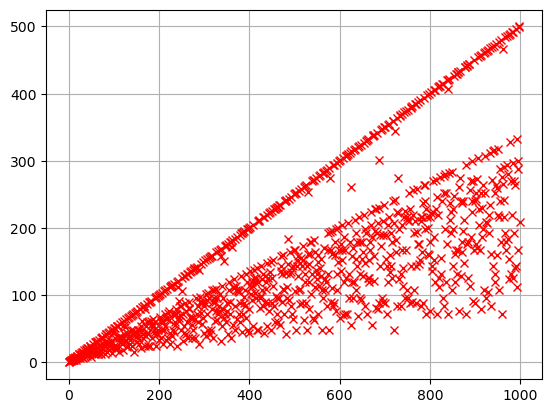
\includegraphics[scale=0.7]{images/2023-02-13-num_quad_residues.png}
\end{figure}


There is a simple criterion by Euler for deciding whether an integer $a$ is a quadratic residue of a given prime p.

\begin{theorem}
Let $p$ be an odd prime and $\gcd(a,p)=1$. Then $a$ is a quadratic residue of $p$ iff

\bee
a^{(p-1)/2} \equiv 1 \mod p
\eee
\end{theorem}

Suppose that $a$ is a quadratic residue of $p$ and $x_1$ is a solution, so that $x_1^2 \equiv a \mod p$. Because $\gcd(a,p) = 1$, we also have $\gcd(x_1,p) = 1$. We can therefore use Fermat's theorem (see entry \ref{2020-12-09:entry}) to obtain

\bee
a^{(p-1)/2} \equiv (x_1^2)^{(p-1)/2} \equiv x_1^{p-1} \equiv 1 \mod p
\eee

For the opposite direction, assume that the congruence $a^{(p-1)/2} \equiv 1 \mod p$ holds and let $r$ be a primitive root of $p$. Then $a \equiv r^k \mod p$ for some integer $k$ with $1 \leq k \leq p-1$. It follows that

\bee
r^{k(p-1)/2} \equiv a^{(p-1)/2} \equiv 1 \mod p
\eee

By theorem \ref{2021-03-02:th0}, the order of $r$ (namely, $p-1$) must divide the exponent $k(p-1)/2$ which implies that $k$ is an even integer which we can express as $k = 2j$. Therefore,

\bee
(r^j)^2 = r^{2j} = r^k \equiv  a \mod p
\eee

which makes the integer $r^j$ a solution of $x^2 \equiv a \mod p$. This proves that $a$ is a quadratic residue of the prime $p$. \qed

If $p$ is (as always) an odd prime and $\gcd(a,p) = 1$, Fermat's theorem states that

\bee
a^{p-1} \equiv 1 \mod p \rightarrow a^{p-1} - 1 \equiv 0 \mod p
\eee

We can factor this as

\bee
a^{p-1} - 1 \equiv \left(a^{(p-1)/2} - 1\right)\left(a^{(p-1)/2} + 1\right) \equiv 0 \mod p
\eee

and for this to hold, either

\bee
a^{(p-1)/2} \equiv 1 \mod p \qquad a^{(p-1)/2} \equiv -1 \mod p
\eee

but not both. If both congruences held simultaneously, we would have $1 \equiv -1 \mod p$, and this would imply $p | 2$ (because the difference between $1$ and $-1$ is two - check for e.g. $p=4$), but would conflict the hypothesis. A quadratic nonresidue does not satisfy $a^{(p-1)/2} \equiv 1 \mod p$ (see previous theorem), it must therefore satisfy $a^{(p-1)/2} \equiv -1 \mod p$.

We can collect this in another theorem.

\begin{theorem}\label{2023-02-13:th2}
Let $p$ be an odd prime and $\gcd(a,p)=1$. Then $a$ is a quadratic residue iff

\bee
a^{(p-1)/2} \equiv 1 \mod p
\eee

and a quadratic nonresidue iff

\bee
a^{(p-1)/2} \equiv -1 \mod p
\eee

\end{theorem}


There is another pprof due to Dirichlet but we skip this here.

Euler’s criterion is not a practical test for determining whether a given integer is or is not a quadratic residue; the calculations involved are too cumbersome unless the modulus is small.

\paragraph{Exercise 1.} We are given $6x^2 + 5x + 1 \equiv 0 \mod p$ and shall show that it has a solution for every prime (even though $6x^2 + 5x + 1$ has no solution over the integers). We have $d = 25 - 4 \cdot 6 \cdot 1 = 1$ and therefore

\bee
y^2 \equiv 1 \mod p \rightarrow y = 1, p-1
\eee

We now need to solve the linear congruence $12x \equiv y-5 \mod p$. For $y = 1$ this becomes $12x \equiv p-4 \mod p$. Using theorem \ref{2020-11-25:th1}, we have $d = \gcd(12, p) = 1$ and the linear congruence has a solution iff $d | b \rightarrow 1 | p-4$ which trivially holds. For $y = p-1$ we have $12x \equiv p-6 \mod p$ and this also has always a solution by the same reasoning. \qed.


\subsection{Legendre Symbols}

We start with the definition of the \emph{Legendre symbol $(a/p)$}. If $p$ is an odd prime and $\gcd(a,p)=1$, the Legendre symbol $(a/p)$ is defined as
 
\bee
(a/p) = \begin{cases} 1 \quad &\text{if $a$ is a quadratic residue of $p$} \\
-1 \quad &\text{if $a$ is a quadratic nonresidue of $p$} \end{cases}
\eee 
 
We call $a$ the numerator and $p$ the denominator of $(a/p)$.

\paragraph{Example.} Looking at our running example with $p=13$, we have $(1/13) = (3/13) =(4/13) = (9/13) = (10/13) = (12/13) = 1$ as these are all the quadratic residues, and $(2/13) = (5/13) = (6/13) = (7/13) = (8/13) = (11/13) = -1$ as these are all the quadratic nonresidues. \qed

The following theorem summarizes some facts about Legendre symbols.

\begin{theorem}
	\label{2023-02-13:th3}
Let $p$ be an odd prime and $a, b$ integers that are relatively prime to $p$. Then the Legendre symbol has the following properties:

\begin{enumerate}
	\item If $a \equiv b \mod p$, then $(a/p) = (b/p)$.
	\item $(a^2/p) = 1$
	\item $(a/p) \equiv a^{(p-1)/2} \mod p$
	\item $(ab/p) = (a/p)(b/p)$
	\item $(1/p) = 1$ and $(-1/p) = (-1)^{(p-1)/2}$
	\item $(ab^2/p) = (a/p)(b^2/p) = (a/p)$
\end{enumerate}
\end{theorem}

Proofs: For 1), we observe that if $a \equiv b \mod p$, then the congruences $x^2 \equiv a \mod p$ and $x^2 \equiv b \mod p$ have exactely the same solutions if any. Thus, $x^2 \equiv a \mod p$ and $x^2 \equiv b \mod p$ are both solvable or neither one has a solution. This is reflected in the statement $(a/p) = (b/p)$.

For 2), we observe that the integer $a$ satisfies $x^2 \equiv a^2 \mod p$ and therefore $(a/p) = 1$.

Part 3) is just a restatement of \ref{2023-02-13:th2}.

For part 4) we use the definition of 3): $(ab/p) = (ab)^{(p-1)/2} = a^{(p-1)/2} b^{(p-1)/2} = (a/p)(b/p)$.

Part 5) can be obtained from 3) by setting $a=1$ and $a=-1$, respectively.

And finally 6) can be obtained by combining 2) and 4). \qed

The second part of 5) can be used to obtain a result for primes having special forms. If $p$ has the form $p = 4k+1$, then $(p-1)/2 = 2k$ which is even and therefore $(-1/p) = (-1)^{2k} = 1$. In a similar spirit, for $p = 4k+3$, we have $(p-1)/2 = 2k+1$ which is odd and therefore $(-1/p) = -1$. We can combine this as

\bee
(-1/p) = \begin{cases} 1 \quad & p \equiv 1 \mod 4 \\
-1 \quad & p \equiv 3 \mod 4 \end{cases} \qed
\eee

As a consequence of part 4, we have that the product of two quadratic nonresidues yields a quadratic residue. For if $(a/p) = (b/p) = -1$, then

\bee
(ab/p) = (a/p)(b/p) = 1 \qed
\eee


The next theorem to tackle is about the number of quadratic residues and nonresidues.

\begin{theorem}
If $p$ is an odd prime, then

\bee
\sum_{a=1}^{p-1} (a/p) = 0	
\eee	

Therefore, there are $(p-1)/2$ quadratic residues and $(p-1)/2$ quadratic nonresidues.
\end{theorem}

Let $r$ be a primitive root of $p$ and from previous entries we know that we can express $a$ in terms of this primitive root: $r^k \equiv a \mod p$. Let's calculate $(a/p)$ as

\bee
(a/p) = \equiv a^{(p-1)/2} \mod p \equiv (r^k)^{(p-1)/2} \mod p = (r^{(p-1)/2})^k \mod p \equiv (-1)^k \mod p
\eee

where, because $r$ is a primitive root of $p$, $r^{(p-1)/2} \equiv -1 \mod p$. Both $(a/p)$ and $(-1)^k$ can attain only $-1$ and $1$; therefore, equality holds in the above equation (instead of "only" $\equiv$). Adding up the Legendre symbols yields,

\bee
\sum_{a=1}^{p-1} (a/p) = \sum_{k=1}^{p-1} (-1)^k = 0 \qed
\eee

We have a corollary: The quadratic residues of an odd prime $p$ are congruent modulo $p$ to the even powers of a primitive root $r$ of $p$; the quadratic nonresidues are congruent to the odd powers of $r$.

\paragraph{Example.} The odd prime $p=13$ has a primitive root $r=2$. According to the corollary, even powers of $r$ yield the quadratic residues, and odd powers yields the quadratic nonresidues.

The quadratic residues are $1, 3, 4, 9, 10, 12$ and the even powers of $r=2$ are

\begin{align*}
& 2^0 \equiv 1 \mod 13, 2^2 \equiv 4 \mod 13, 2^4 \equiv 3 \mod 13 \\
& 2^6 \equiv 12 \mod 13 2^8 \equiv 9 \mod 13, 2^{10} \equiv 12 \mod 13
\end{align*}

The quadratic nonresidues are therefore $2, 5, 6, 7, 8, 11$ and the odd powers of $r=2$ are

\begin{align*}
& 2^1 \equiv 1 \mod 13, 2^3 \equiv 8 \mod 13, 2^5 \equiv 6 \mod 13 \\
& 2^7 \equiv 11 \mod 13 2^9 \equiv 5 \mod 13, 2^{11} \equiv 7 \mod 13
\end{align*}

\qed

We next have Gauss' Lemma.

\begin{theorem}
	\label{2023-02-13:th4}
Let $p$ be an odd prime and $\gcd(a,p)=1$. We define the set $S = \{a, 2a, 3a, \cdots, \frac{p-1}{2}a \}$ which has $(p-1)/2$ elements. Now let $n$ denote the number of integers in $S$ whose remainders upon division by $p$ exceeds $p/2$. Then we have

\bee
(a/p) = (-1)^n
\eee

\end{theorem}

\paragraph{Example.} For $p=13$ and $a=5$, we have $(p-1)/2 = 6$ and the set $S$ becomes

\bee
S = \{5, 10, 15, 20, 25, 30\}
\eee

If we take the elements $\mod 13$, we have $\{5, 10, 2, 7, 12, 4\}$ and three of them ($7, 10, 12$) are greater than $p/2 = 13/2=6.5$, therefore $n=3$. According to the theorem $(5/13) = (-1)^3 = -1$ and this corresponds to the fact that $5$ is a quadratic nonresidual. \qed

\paragraph{Proof.} We start by observing that due to $\gcd(a,p)=1$, none of the $(p-1)/2$ numbers in $S$ is congruent to zero
and no two are congruent to each other modulo $p$. Denote by $r_1, \ldots, r_m$ the remainders upon division by $p$ which are smaller than $p/2$ and denote by $s_1, \ldots, s_n$ the $n$ remainders upon division by $p$ which are larger than $p/2$ (and the theorem states that $(a/p) = (-1)^n$). 

Since the set $S$ has $(p-1)/2$ elements and therefore also $(p-1)/2$ remainders, we have $m + n = (p-1)/2$ and the numbers

\bee
r_1, \ldots, r_m \quad \text{and} \quad p - s_1, \ldots, p - s_m
\eee

are all positive and less than $p/2$.

We want to show that these numbers are the integers $1, 2, \ldots, (p-1)/2$ but in a different order (in our example from above, the $r_i$ are $2, 4, 5$ and the $p - s_i$ are $1, 3, 6$). We start with showing that the numbers are all distinct. It suffices to show that no $p - s_i$ is equal to any $r_j$. We prove by contradiction and assume 

\bee
p - s_i = r_j
\eee

for some choice of $i, j$. Then there exist integers $u, v$ with $1 \leq u, v \leq (p-1)/2$ which satisfy $s_i \equiv u a \mod p$ and $r_j \equiv v a \mod p$ and therefore

\bee
(u+v)a \equiv r_i + s_i = p \equiv 0 \mod p
\eee

and from this follows $u + v \equiv 0 \mod p$. But this cannot be, because we have restricted $u, v$ to $1 \leq u, v \leq (p-1)/2$ (looking at the example from above, we have $(p-1)/2 = 6$, therefore $1 \leq u,v \leq 6$ and $0 + 0 = 0 \not\equiv 0 \mod 13$ nor $6 + 6 = 12 \not\equiv 0 \mod 13$).


To conclude, the $(p-1)/2$ numbers $r_1, \ldots, r_m, p - s_1, \ldots, p - s_m$ are all distinct, positive, and smaller than $(p-1)/2$. Therefore, they must be equal to the numbers $1, 2, \ldots, (p-1)/2$ but in a different order. Multiplying them together yields

\begin{align*}
\left( \frac{p-1}{2} \right) ! &= r_1 \cdots r_m (p-s_1)\cdots (p-s_n) \\
&\equiv r_1 \cdots r_m (-s_1)\cdots (-s_n) \mod p \\
&\equiv(-1)^n r_1 \cdots r_m s_1\cdots s_n \mod p
\end{align*}

However, we know that the $_1, \ldots, r_m, s_1\ldots s_n$ are congruent modulo-$p$ to $a, 2a, \ldots, \frac{p-1}{2}a$  in some order. Therefore 

\begin{align*}
\left( \frac{p-1}{2} \right) ! &\equiv (-1)^n a \cdot 2a \cdots \frac{p-1}{2}a \mod p \\
&\equiv (-1)^n a^{(p-1)/2} \frac{p-1}{2}a \mod p
\end{align*}

Because $\frac{p-1}{2}a \mod p$ is relatively prime to $p$, we can cancel it on both sides and we arrive at

\bee
1 \equiv (-1)^n a^{(p-1)/2}  \mod p \\
\eee

or

\bee
(-1)^n  \equiv a^{(p-1)/2}  \mod p \\
\eee

But the RHS is exactely $(a/p)$ and we conclude that

\bee
(a/p) \equiv (-1)^n \mod p \qed
\eee

We can use Gauss' lemma for some interesting results.

\begin{theorem}
	If $p$ is an odd prime, then

	\bee
		(2/p) = \begin{cases}
			1 & \text{if } p \equiv 1 \mod 8 \text{ or } p \equiv 7 \mod 8 \\
			- 1 & \text{if } p \equiv 3 \mod 8 \text{ or } p \equiv 5 \mod 8
		\end{cases}
	\eee
\end{theorem}

Proof is omitted. We can use this theorem to prove that there are infinitely many primes of the form $8k-1$ (proof omitted). As a corollary, we have

\begin{theorem}
	If $p$ is an odd prime, then

	\bee
	(2/p) = (-1)^{(p^2-1)/8}
	\eee
\end{theorem}

and finally

\begin{theorem}
	If $p$ and $2p+1$ are both odd primes, then the integer

\begin{equation}
	(-1)^{(p-1)/2} \cdot 2
\end{equation}

is a primitive root of $2p+1$.

\end{theorem}

As an exmaple, we consider $p = 5$ with $2p+1=11$ being an odd prime. Therefore $(-1)^{(p-1)/2} \cdot 2 = 2$ is a primitive root of $11$. Perhaps more interesting is the case $p=11$ ($2p+1=23$ being an odd prime) from which we conclude that $(-1)^{(p-1)/2} \cdot 2 = -2 \equiv 21 \mod 23$ is a primitive root of $23$.

We can prove this by denoting $q=2p+1$ and distinguish two cases: $p \equiv 1 \mod 4$ and $p \equiv 3 \mod 4$. 

Let's start with $p \equiv 1 \mod 4$ (i.e. $p=5, 9, 13,\ldots = 4k+1$). We first observe that $(-1)^{(p-1)/2} \cdot 2 = (-1)^{2k} \cdot 2 = 2$. Because $\phi(q) = q-1 = 2p$ (the first because $q$ is a prime and the second from the definition of $q$), the order of $2 \mod q$ is either $1, 2, , p$, or $2p$ \todo{why?}. Using property 3) of theorem \ref{2023-02-13:th3}, we have

\bee
(2/q) \equiv 2^{(q-1)/2} = 2^p \mod q
\eee

With $p \equiv 1 \mod 4$, we have $q \equiv 3 \mod 8$ and therefore $(2/q) = -1$ \todo{why}. It follows that $2^p \equiv -1 \mod q$ and therefore $2$ cannot have order $p \mod q$. The order of $2$ being neither $1$ or $2$ ($2^2 \equiv 1 \mod q$ implies that $q |3$ and this contradicts the prime assumption), nor $p$, we conclude that the order of $2 \mod q$ is $2p$ and therefore $2$ is a primitive root of $q$.

The other case is $p \equiv 3 \mod 4$ (i.e. $p=7, 11, 15,\ldots = 4k+3$). and yields $(-1)^{(p-1)/2} \cdot 2 = (-1)^{2k+1} \cdot 2 = -2$. Therefore

\begin{equation}
	(-2)^p \equiv (-2/q) = (-1/q)(2/q) \mod q
\end{equation}

With $p \equiv 3 \mod 4$, we have $q \equiv 7 \mod 8$ and therefore $(-1/q) = -1$ and we therefore have $(2/q) = 1$ which leads to $(-2)^p \equiv -1 \mod q$. We can follow an argument simialr to the first case, and conclude that $-2$ is a primitive root of the prime $2p+1$. \qed

There is a another result of the same character: If both $p$ and $4p+1$ are primes, then $2$ is a primitive root of $4p+1$.

An odd prime $p$ such that $2p+1$ is also a prime is called a \emph{Germain prime}, after the French number theorist Sophie Germain (1776–1831). An unresolved problem is to determine whether there exist infinitely many Germain primes.





\subsection{Quadratic Reciprocity}

Let $p$ and $q$ be distinct odd primes, so that both of the Legendre symbols $(p/q)$ and $(q/p)$ are defined. We ask whether the value of $(p/q)$ can be determined if that of $(q/p)$ is known. To put the question more generally, is there any connection at all between the values of these two symbols?

It turns out there is and it is the Quadratic Reciprocity Law,

\bee
(p/q)(q/p) = (-1)^{\frac{p-1}{2} \frac{q-1}{2} }
\eee

\paragraph{Example.} Let's try this with a simple example; $p=13, q=17$. Starting with $q=17$, we have that $p=13$ is a quadratic residue and therefore $(13/17) = 1$. The other way round, also $17 \equiv 4 \mod 13$ is a quadratic residue of $13$, therefore $(17/13) = 1$. Their product is therefore $(13/17) (17/13) = 1$.

Comparing with the quadratic reciprocity law, we have

\bee
(-1)^{\frac{p-1}{2} \frac{q-1}{2}} = (-1)^{6 \cdot 8} = (-1)^{48} = 1
\eee

We can also do this in Python,

\begin{verbatim}
from sympy.ntheory import quadratic_residues
from sympy.ntheory import legendre_symbol

quadratic_residues(13)
Out[3]: [0, 1, 3, 4, 9, 10, 12]

quadratic_residues(17)
Out[4]: [0, 1, 2, 4, 8, 9, 13, 15, 16]

legendre_symbol(13, 17)
Out[5]: 1

legendre_symbol(17, 13)
Out[6]: 1

(-1)**(6*8)
Out[7]: 1
\end{verbatim}



%%% Local Variables:
%%% mode: latex
%%% TeX-master: "journal"
%%% End:
